\section{Introduction}

This chapter introduces a multi-block generalisation of ADMM, suitable for inference over sensor networks. We propose a decentralised solver for recovering a signal from a set of compressive measurements, independently made at each node. We improve over the model of \cite{Zhang2011b} by not requiring the use of a Fusion Centre to do the reconstruction - this is replaced by softhresholded gradient descent and local communications between neighbouring nodes to recover the signal. 

We also improve on the work of \cite{mota2013d}, by providing explicit, closed form, iterates for a series of functionals commonly used in Compressive Sensing - as opposed to relying on a slow intermediate optimisation algorithm to find intermediate points. To derive our algorithm, we give new proofs of ideas found in \cite{mota2013d}

The structure of the chapter is as follows: we give an overview of the (vector) sensing model at each node, and how the global sensing model decomposes into a collection of individual sensing problems at each node. 

We then give a derivation of the new algorithm for composite smooth and non-smooth objective functions. In the derivation we form a global objective, and show how it can be decomposed into a collection of separate objectives. We give new proofs of ideas in \cite{mota2013d} - specifically we show how the objective decomposes over edges between nodes, and thus the global objective can be written as a sum of local objective functions at each node. Thus each node can execute a series of simple operations, built up from matrix vector multiplies and component wise thresholding, along with a single step of local communication at each iteration.

We demonstrate the general algorithm on two widely used objective functions in compressive sensing - the LASSO (both with \(\ell_1\) and \(\ell_0\) regularisation) (see \eqref{program:lasso}) and the Dantzig Selector (see \eqref{program:danzig}). We demonstrate recovery on synthetic random signals.

We then extend the vector algorithm to matrix sensing problems, and demonstrate recovery in the multiple measurement vector (MMV) case. We demonstrate signal recovery with a distributed Modulated Wideband converter model. We show that the MMV-LASSO recovery achieves adequate performance for spectrum sensing, both in terms of reconstruction accuracy and in terms of signal undersampling. 


\section{Constrained Optimisation on Graphs}\label{sec:opt-on-graphs}

We model the network of sensors as an undirected graph \(G = \left(V,E\right)\), where \(V = \{1, \ldots, J\}\) is the set of vertices, and \(E = V \times V\) is the set of edges. An edge between nodes \(i\) and \(j\) implies that the two sensors can communicate. The set of nodes that node \(i\) can communicate with is written \(\mathcal{N}_i\) and the degree of node \(i\) is \(D_i = |\mathcal{N}_i|\). 

We are considering a distributed variation of the following model:

\begin{equation}
y = A x + n
\end{equation}
\label{eq:system}

Where, \(y, n\in \re^{p}\), \(x \in \re^n\), \(A\in \re^{p \times n}\). This is a standard scenario. Individually nodes make the following measurements:

\begin{equation}
\vec{y}_r = \vec{A}_r\vec{x} + \vec{n}_r
\end{equation}

where \(\vec{A}_r\) is the \(r^{th} \) row of the sensing matrix from \eqref{eq:system}, and \eqref{eq:system} is formed by concatenating the individual nodes' measurements together.

We assume that a proper colouring of the graph is available: that is, each node is assigned a number from a set \(C = \{1 \ldots c \} \), and no node shares a colour with any neighbour. This is so that nodes may communicate in colour order, as opposed to communicating individually thus reducing the total number of communication rounds required. 

To find the \(\vec{x}\) we are seeking (the solution to the linear system \eqref{eq:system}), to each node we give a copy of \(\vec{x}, \vec{x}_p\) and we constrain the copies to be identical across all edges in the network. Each node, thus has a separate optimisation to solve, subject to the constraint that it is consistent with its neighbours.

The problem then is to solve:

\begin{align}
\argmin_{\bar{x}} \sum_{c=1}^C \sum_{j \in C_c} f\left(x_j\right) + \frac{\lambda}{J} g\left(x_j\right) \nonumber \\ 
\text{ s.t } x_i = x_j \text{ if } \{i,j\} \in E \nonumber \\
\text{ and } x_i = z_i \text{ } \forall i \in \{1, \ldots, C\}
\label{constrainedbp}
\end{align}

We can write the global optimisation variable as \(\bar{x}\), which collects together \(C\) copies of a \(n\times 1\) vector \(\vec{x}\):

\begin{definition}
We define vectors \(x_c\), where \(c = 1,\ldots , C\) and write the vector of length \(nJ\):
\begin{equation}
\bar{x} = \sum_{c=1}^C w_c \otimes x_c = \left[x_{c(1)}^T, \ldots	, x_{c(J)}^T\right]^T
\label{barxc}
\end{equation}
where \(w_{c(i)} = \mathbb{I}(c(i) = c)\), \(\mathbb{I}\) is the indicator function, and we have written \(c(i)\) for the colour of the \(i\)th node.
\end{definition}

These constraints can be written more compactly by introducing the node-arc incidence matrix B: a \(V\) by \(E\) matrix where each column is associated with an edge \(\left(i,j\right) \in E\) and has \(1\) and \(-1\) in the \(ith\) and \(jth\) entry respectively. Figures \eqref{efig:ex-network} and \eqref{fig:incidence-matrix} show examples of a network and it's associated incidence matrix.

The constraint \(x_i = x_j \text{ if } \{i,j\} \in E \) can now be written 

\begin{equation}
\sum_{c=1}^C\left(B_c^T \otimes I_n\right)\bar{x}_c = 0
\label{compact-constraints}
\end{equation}

note that \(\left(B^T\otimes I_n \right) \in \re^{nE \times nJ}\). Together \eqref{barxc} and \eqref{compact-constraints}, suggests that the problem \eqref{constrainedbp} can be re-written as:

\begin{align}
\argmin_{\bar{x}} \sum_{c=1}^C \sum_{j \in C_c} f\left(x_j\right) + \frac{\lambda}{J} g\left(z_j\right)
\nonumber \\
\text{ s.t. } \sum_{c=1}^C\left(B_c^T \otimes I_n\right)\bar{x}_c = 0 \nonumber \\
\text{ and } \bar{x}_c - \bar{z}_c = 0
\label{constrainedbp1}
\end{align}

where \(\beta = \frac{\lambda}{J}\).

The global Augmented Lagrangian \cite{Boyd2010a}
 for the problem \eqref{constrainedbp1} can be written down as:

\begin{align}
L_\rho = \sum_{c=1}^C  \bigg( \sum_{j \in c} & f\left(x_j\right) + \frac{\lambda}{J} g\left(z_j\right)  + \nonumber \\ & + \theta^T\left(\bar{x}_j - \bar{z}_j\right)  +  \frac{\rho}{2}\vectornorm{\bar{x}_j-\bar{z}_j}_2^2 \bigg) + \nonumber \\  & + \eta^T\left(B_c^T \otimes I_n\right)\bar{x}_c + \frac{\rho}{2}\vectornorm{\sum_{c=1}^C\left(B_c^T \otimes I_n\right)\bar{x}_c}_2^2
\label{aug-lagrange}
\end{align}

This is, superficially, similar to the Augmented Lagrangian for the Lasso problem \cite{Boyd2010a}[Section 6.4]. That is, the terms indexed by \(j\) are a straightforward Lasso problem, constrained by edge-wise variables (indexed by \(c\)) forcing consistency across the network. However, the problem (as currently written) is not separable across the edges of the network (in the sense that the Lagrangian \eqref{aug-lagrange} is composed only of terms with the subscript \(j\)) as the final and penultimate term represent the constraint that the nodes agree on their estimates across edges. 

To make it possible that \ref{aug-lagrange} can be posed  as a constrained optimisation problem at each node, we introduce the following variable (so that the the final term of \ref{aug-lagrange} is separable across edges of the graph):

\begin{definition}
\begin{align*}
u &:= \left(B^T \otimes I_n\right)\bar{x} \\
& = \left(B^T \otimes I_n\right)\sum_{c=1}^C w_c \otimes x_c \\
& = \sum	_{c=1}^C B_c^T\otimes x_c
\end{align*}
where we have used the definition \eqref{barxc} in the second line, and the property of Kronecker products \((A\otimes C)(B \otimes D) = (AB \otimes CD)\) between the second and third lines, and we write \(B_c = w_c^TB\).
\end{definition}

\begin{figure}[h]
\centering
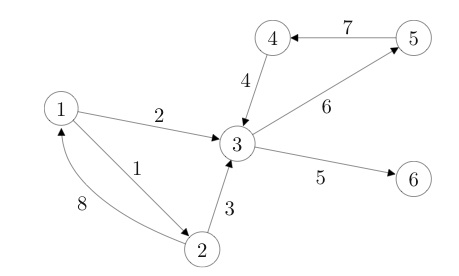
\includegraphics[height = 5 cm]{network-ex-incidence-mat.jpg}
\caption{An example of a network}
\label{efig:ex-network}
\end{figure}

\begin{figure}[h]
\centering
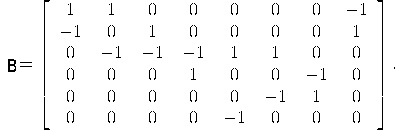
\includegraphics[height = 3 cm, width = 7cm]{ex-incidencematrix1.png}
\caption{The incidence matrix associated with Figure \eqref{efig:ex-network}}
\label{fig:incidence-matrix}
\end{figure}

The terms \(\|\sum_{c=1}^C\left(B_c^T \otimes I_n\right)\bar{x}_c\|^2\) and \( \eta^T\left(B_c^T \otimes I_n\right)\bar{x}_c \) of \eqref{aug-lagrange}, can be decomposed across edges, using the following lemma:

\begin{lemma}[Edge Decomposition]
\begin{equation}
\vectornorm{\sum_{c=1}^C\left(B_c^T \otimes I_n\right)\bar{x}_c}^2 = \sum_{j \in C_1}\left( D_j\vectornorm{x_j}_2^2 - \sum_{k \in N_j} x_j^Tx_k\right)
\end{equation}

and

\begin{equation}
\eta^T\sum_{c=1}^C\left(B_c^T \otimes I_n\right)\bar{x}_1 = \sum_{l\in C_c} \sum_{m\in N_l}sign\left(m-l\right)\eta_{ml}^T x_l
\end{equation}

where \(\eta\) is decomposed edge-wise: \(\eta = \left(\ldots, \eta_{ij},\ldots\right)\), such that \(\eta_{i,j} = \eta_{j,i}\), and is associated with the constraint \(x_i = x_j\).


\begin{proof}

\begin{align*}
u^Tu &= \sum	_{c_1=1}^C \sum	_{c_2=1}^C  \left(B_{c_1} \otimes x_{c_1}^T\right) \left(B_{c_2}^T \otimes x_c\right) \\
&= \sum_{c_1, c_2} B_{c_1}B_{c_2}^T \otimes x_{c_1}^Tx_{c_2}
\end{align*}

\(BB^T\) is a \(J \times J\) matrix, with the degree of the nodes on the main diagonal and \(-1\) in position \(\left(i,j\right)\) if nodes \(i\) and \(j\) are neighbours (i.e \(BB^T\) is the graph Laplacian). Hence, since we can write \(B_{c_1}B_{c_2}^T = w_{c_1}^TBB^Tw_{c_2}\), the trace of \(B_{c_1}B_{c_1}^T\) is simply the sum of the degrees of nodes with colour 1. 

For \(c_1 \neq c_2\),  \(B_{c_1}B_{c_2}^T\) corresponds to an off diagonal block of the graph Laplacian, and so counts how many neighbours each node with colour 1 has.

Finally, note that \(\eta \in \re^{nE}\) and can be written:

\begin{equation}
\eta = \sum_{c=1}^C w_c \otimes \eta_c
\end{equation}
where \(\eta_c\) is the vector of Lagrange multipliers associated across edges from colour \(c\). Now

\begin{align*}
\eta^Tu = \sum_{c_1=1}^C\sum_{c_2=1}^C w_{c_1}Bw_{c_2} \otimes \eta_{c_1}^Tx_c
\end{align*}
by the properties of Kronecker products, and the definition of \(B_c\). For \(c_1=c_2\), \(\eta^Tu\) is zero, as there are no edges between nodes of the same colour b definition. For \(c_1\neq c_2\), \(\eta^Tu\) counts the edges from \(c_1\) to \(c_2\), with the consideration that the edges from \(c_2\) to \(c_1\) are counted with opposite parity.
\end{proof}
\end{lemma}

Thus, we are able to write \eqref{aug-lagrange} as:

\begin{align}
L_\rho = \sum_{c=1}^C\sum_{j \in C_c} &\left( f\left(x_j\right) + \beta g\left(z_j\right)\right) + \nu^Tx_j \nonumber \\
& \text{        } \theta\left(x_j - z_j\right) + \frac{\rho}{2}D_i\vectornorm{x_j}^2 + \frac{\rho }{2}\|x_j-z_j\|^2
\label{generic-iterations}
\end{align}

where we have defined:

\begin{equation}
\nu_i = \left(\sum_{k \in \mathcal{N}_i} sign\left(k-i\right)\eta_{\{i,k\}} - \rho x_k \right)
\end{equation}

this is a re-scaled version of the Lagrange multiplier, \(\eta\). 

Then by differentiating \eqref{generic-iterations} with respect to \(x_j\) and \(z_j\) we  can find closed forms for the updates as:

\begin{theorem}
\begin{align}
x_j^{k+1} &:= \mathrm{Prox}_f \left( z_j^k - \theta_j^k\right)\\
z_j^{k+1} &:= \mathrm{Prox}_g \left( x_j^{k+1} + \theta_j^k\right)
 \\
\theta_j^{k+1} &:= \theta_j^{k} + \rho \left(x^{k+1}-z^{k+1}\right) \\
\eta_j^{k+1} &:= \eta_j^k + \rho\left(\sum_{m \in N_j} z_m^k - z_j^k\right)
\label{dadmm_algo}
\end{align}
\end{theorem}

This algorithm can be thought of as follows: each node performs an iteration of (non multi-block) ADMM - i.e. each node solves an approximate Gaussian least-squares problem and then soft-thresholds - and then exchanges the result of this computation with its one-hop neighbours. This explains the inclusion of an extra Lagrange multiplier: the multiplier \(\theta\) controls how far each node moves from its previous estimate in each iteration, whilst the multiplier \(\eta\) enforces consistency between nodes. Note that there is no communication of data between the nodes - only the result the computation in each round.

\subsection{DADMM-Lasso}\label{sec:lasso-algo}

In this section we derive a version of algorithm \ref{dadmm_algo} applied to the specific problem of sparse estimation with the LASSO (repeated here for convenience):

\begin{equation}
L = \frac{1}{2} \vectornorm{Ax-y}_2^2 + \lambda\vectornorm{x}_1
\label{LASSO-chapter5}
\end{equation}

The Proximity operators of \(f = \frac{1}{2} \vectornorm{Ax-y}_2^2\) and \(\lambda\vectornorm{x}_1\), are 

\begin{equation}
\mathrm{Prox}_f\left(x\right) = \left(A^TA + \rho I\right)^{-1}\left(A^Ty - x\right)
\end{equation}

and 

\begin{equation}
\mathrm{Prox}_g\left(x\right) = S_\gamma\left(x\right)_i 
\end{equation}

respectively. We can write the Lagrangian for this problem as:

\begin{align}
L_\rho = \sum_{c=1}^C\sum_{j \in C_c} & \frac{1}{2} \vectornorm{A_j x_j -y_j}_2^2  + \beta\vectornorm{x_j}_1  + \nu^Tx_j  + \\
& \text{        } \theta\left(x_j - z_j\right) + \frac{\rho}{2}D_i\vectornorm{x_j}^2 + \frac{\rho}{2}\|x_j-z_j\|^2
\label{dadmm-lasso-lag}
\end{align}

and by differentiating \eqref{dadmm-lasso-lag} We finally arrive at the following algorithm:

\begin{corollary}
\begin{align}
x_j^{k+1} &:= \left(A_j^TA_j + (\rho D_J + 1) I\right)^{-1}\left(A_j^Ty_j +  z^k - \theta^{kT} - \nu^{kT}\right)\\
z_j^{k+1} &:= S_{\beta/\rho}\left(x_j^{k+1} \right)
 \\
\theta_j^{k+1} &:= \theta_j^{k} + \rho \left(x^{k+1}-z^{k+1}\right) \\
\eta_j^{k+1} &:= \eta_j^k + \rho\left(\sum_{m \in N_j} z_m^k - z_j^k\right)
\label{dadmm_algo_lasso}
\end{align}
\end{corollary}

\subsection{DADMM-MMV}\label{sec:mmv-algo}
In this section we extend our results to the multiple measurement vector (\gls{mmv}) model of \cite{cotter2005sparse}. The model can be summarised as follows:

\begin{equation}
Y = AX + N
\end{equation}

Here, \(Y, N\in \re^{m\times p}\), \(x \in \re^{p\times n}\), \(A\in \re^{m \times n}\)

The \gls{mmv} model is an extension of \eqref{eq:system} where instead of a single sparse vector being estimated, a set of multiple (jointly) sparse vectors are recovered (under the assumption that these vectors share a common set of non-zeros).

The resulting optimisation problem is:

\begin{equation}
\argmin_X \vectornorm{X}_{2,1} \text{ s.t } Y=AX
\label{program:bpmmv}
\end{equation}

which can be recast in unconstrained form as:

\begin{equation}
\argmin_X \frac{1}{2}\vectornorm{AX-Y}_F^2 + \lambda\vectornorm{X}_{2,1}
\label{program:lassommv}
\end{equation}

This can be turned into a distributed optimisation problem, and so solved with \eqref{dadmm_algo}. The augmented Lagrangian for this system is:

\begin{align}
L_\rho = \sum_{c=1}^C\sum_{j \in C_c} & \frac{1}{2} \vectornorm{A_j X_j - Y_j}_F^2  + \beta\vectornorm{X_j}_{2,1}  + \nu^Tx_j  + \\
& \text{        } \theta\left(X_j - Z_j\right) + \frac{\rho}{2}D_i\vectornorm{X_j}^2 + \frac{\rho}{2}\|X_j-Z_j\|^2
\end{align}

and by differentiating we arrive at the following algorithm:

\begin{align}
X_j^{k+1} &:= \left( A_j^T A_j + (\rho D_J + 1) I \right)^{-1}\left(A_j^T Y_j + \rho Z^k - \Theta - N^{kT} \right) \\
Z_j^{k+1} &:= S_{\beta/\rho}\left(X_j^{k+1} \right)
 \\
\Theta_j^{k+1} &:= \Theta_j^{k} + \rho \left(X^{k+1}-Z^{k+1}\right) \\
H_j^{k+1} &:= H_j^k + \rho \left(\sum_{m \in N_j} Z_m^k - Z_j^k\right)
\end{align}

\section{Results} \label{sec:results}

We tested our algorithms on random, simulated, data from two classes: to measure reconstruction quality we used random Gaussian signals, and to create ROC curves we used random uniform signals (fence-post signals). The former was generated with MATLAB's \(mathrm{sprandn}\) function, whilst the latter was generated by selecting uniformly distributed vector components and setting the value of those chosen to unity - all other components are left at zero.

We compared the mean squared error (MSE) of our algorithms with a centralised solver (spgl1). We, investigated the performance of the algorithm with various settings of the regression parameter \(\lambda\), and at various signal-to-noise ratios. 

The MSE was calculated as follows:

\begin{equation}
\frac{\vectornorm{Z^k - Z^*}}{\vectornorm{Z^*}}
\end{equation}

where \(Z^k\) is the result of the algorithm at iteration \(k\), and \(Z^*\) is the optimal solution.

We first tested the algorithm's ability to reconstruct a sparse signal, to what extent this reconstruction is accurate and useful, and how it would compare with a centralised algorithm with access to all the information. We vary the regression parameter \(\lambda\) whilst keeping the \gls{snr} constant. Noise was added to this the system, to more realistically simulate scenarios found 'in the wild'.

Figure \ref{ch5:fig:differentLambda} shows the progress of the algorithm iterations for different values of the regression parameter. It (figure \ref{ch5:fig:differentLambda}) is complemented by figure \ref{ch5:fig:erroriterations} which shows the progress of the algorithm iterations and a centralised solver (spgl11) which has all of the information. Collectively these show that for any given value of \(\lambda\), the algorithm converges to a stable solution. However, some fine tuning of \(\lambda\) may be needed to find an acceptable solution - one in which a node can find a solution at least as good as a central processor with all the information. These figures also display the previously noted \cite{Boyd2010} behaviour that ADMM converges to a good solution in a few iterations, but takes considerably longer to converge to an excellent one.

We then contrasted \(\ell_1\) and \(\ell_0\) regularisation in the distributed algorithm. The results are presented in figure \ref{ch5:fig:l1l0} which shows the algorithm with different regularisation - \(\ell_1\) vs \(\ell_0\). Figure \ref{ch5:fig:l1l0-long} is another similar experiment, but with an extended number of iterations. There is some tension between these two figures, as figure \ref{ch5:fig:l1l0} shows that \(\ell_0\) regularisation is considerably worse than \(\ell_1\) penalisation, whilst figure \ref{ch5:fig:l1l0-long} shows the exact opposite. Qualitatively speaking, we found that \(\ell_1\) regularisation provided more reliable results - in the sense of consistently and predictably finding a good solution. This can be explained by noting that \(\ell_0\) regularised LASSO is a non-convex objective, and whilst it's Prox operator can be computed the algorithm can get stuck in sub-minimal local optima. This is not a problem for \(\ell_1\) regularised LASSO, as for any given \(\lambda\) there is a single minima, which gradient descent algorithms are guaranteed to converge to (however slowly). 

Finally, in the discussion of vector valued problems, we compared our algorithm to that presented in \cite{ling2015dlm}, where a linear approximation to the objective is made to facilitate speedy computation. For clarity the steps of the algorithm are:

\begin{thm}
\begin{align}
x_j^{k+1} &:= x^{k} - \frac{1}{d_i}\left(\nabla f(x) +\rho\left(\sum_{j \in \mathcal{N}_i} x_i - x_j \right) + \theta^k\right)\\
\theta_j^{k+1} &:= \theta_j^{k} + \rho \left(\sum_{j \in \mathcal{N}_i} x_i - x_j \right)
\label{dlm_algo}
\end{align}
\end{thm}

Figures \ref{ch5:dlm1} and \ref{ch5:dlm2} show the results of our experiments: they clearly show our methods are superior -  Both in the sense of converging to a better solution, but also doing this in far fewer iterations (1000 vs 10000 or more). 

We also simulated the MWC system from section \ref{sec:MWC}, and we qualitatively assessed the results of the MMV algorithm \ref{sec:mmv-algo}. The MWC system was simulated, and a the MMV algorithm presented in section \ref{sec:mmv-algo} was used to reconstruct the original signal. As can be seen in figure \ref{ch5:fig:mmv-recon}, the reconstruction is qualitatively similar to the original (pictured in figure \ref{ch5:fig:mmv-orig}). However, the reconstruction fails qualitatively to be better than simply calculating \(A^Ty\) - plotted in figure \ref{ch5:aty}. This could be for a variety of reasons:

\begin{itemize}
\item An incorrect regression parameter \(\lambda_mmv\) was used. Wheras for vector inverse problems - problems where a vector \(x \in \re^n\) is inferred from measurements \(y \in \re^m\) - where the choice of \(\lambda\) is bounded between \(0 \) and \(\vectornorm{A^Ty}_\infty\), with a popular choice being \(\sqrt{2\sigma \log{n}}\), finding an appropriate \(\lambda\) when \(x\) is reshaped into \(X \in \re^{k \times p}\) is unclear.
\item It is inappropriate to try to perform the inversion of a vector valued problem as a matrix valued problem.
\end{itemize}

We think that the problem is a mixture of the two. 

\begin{figure}[h]
\centering
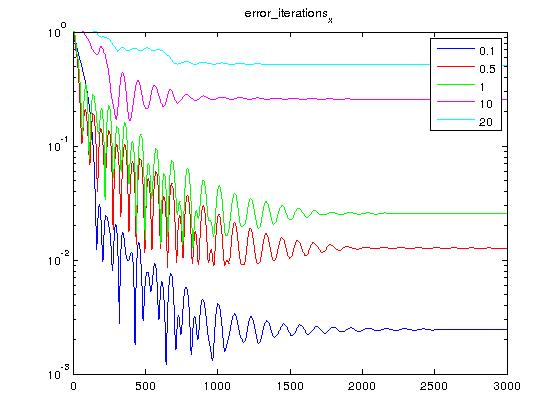
\includegraphics[height = 7.3 cm]{different_lambda.jpg}
\caption{The progress of the distributed solver as a function of the number of iterations, with different values of the regression parameter \(\lambda\)}
\label{ch5:fig:differentLambda}
\end{figure}

\begin{figure}[h]
\centering
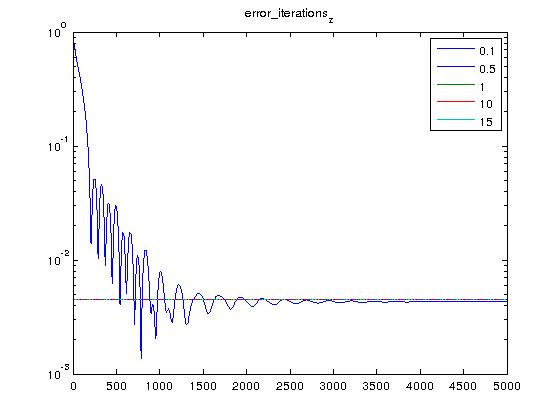
\includegraphics[height = 7.3 cm]{mse_iterations.jpg}
\caption{The progress of a distributed (blue) and a centralised (green) solver as a function of the number of iterations. The value of \(\lambda = 0.1\)}
\label{ch5:fig:erroriterations}
\end{figure}

\begin{figure}[h]
\centering
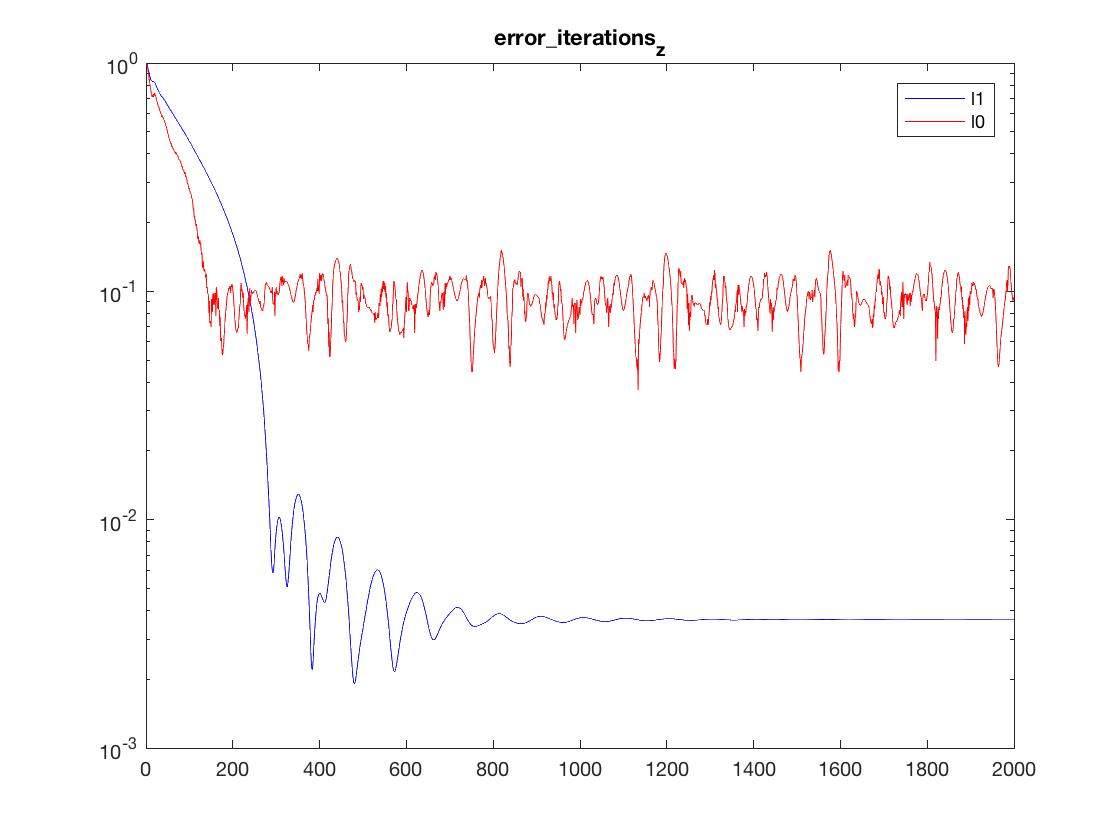
\includegraphics[height = 7.3 cm]{l1vsl0.jpg}
\caption{The progress of the distributed solver with \(\ell_1\) (blue) and \(ell_0\) (red) regularisation as a function of the number of iterations.}
\label{ch5:fig:l1l0}
\end{figure}

\begin{figure}[h]
\centering
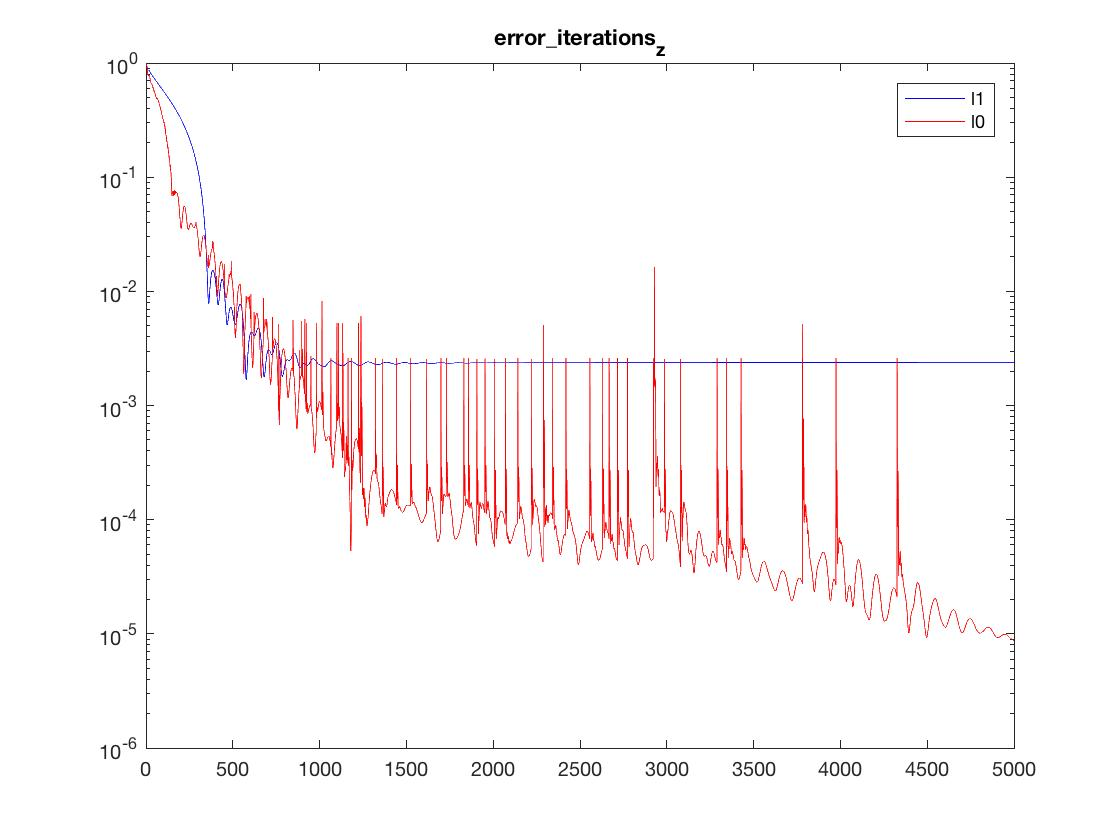
\includegraphics[height = 7.3 cm]{l1vsl0-long.jpg}
\caption{The progress of the distributed solver with \(\ell_1\) (blue) and \(ell_0\) (red) regularisation as a function of the number of iterations. \(\lambda_{\ell_1} = P\sqrt{2\log{n}}\),  \(\lambda_{\ell_0} = 1000\lambda_{\ell_1}\) }
\label{ch5:fig:l1l0-long}
\end{figure}

\begin{figure}[h]
\centering
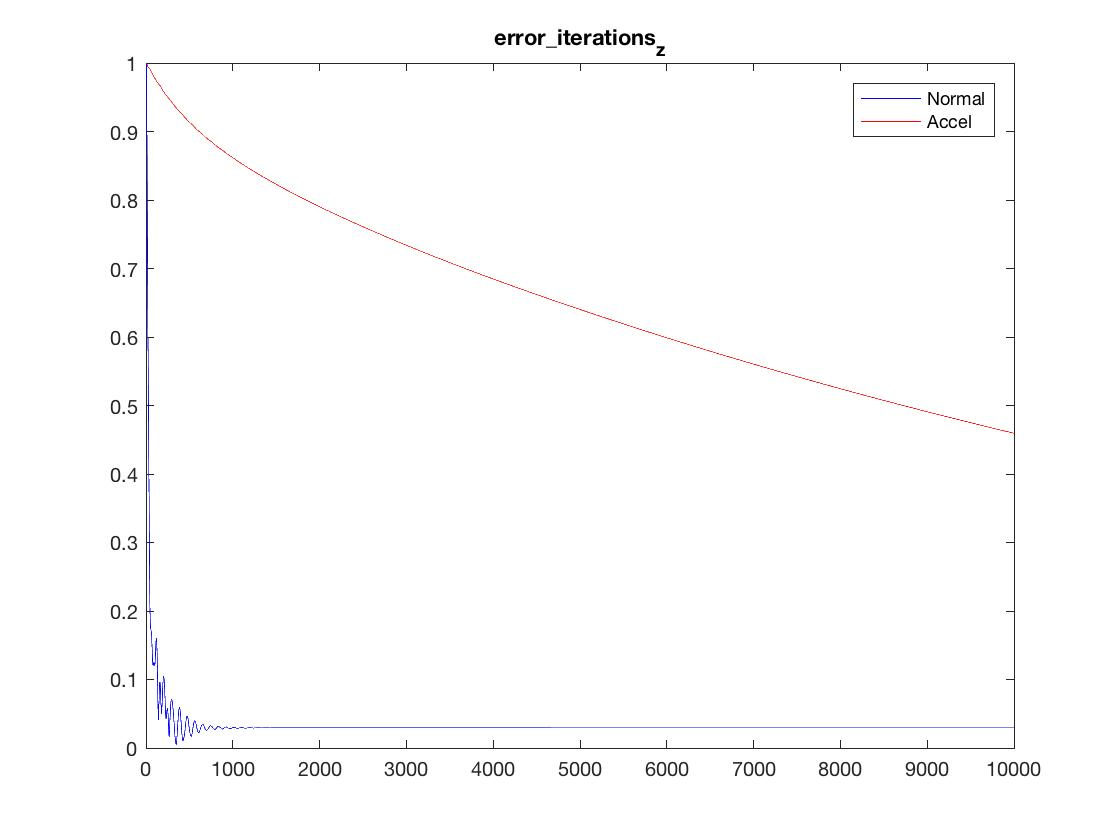
\includegraphics[height = 7.3 cm]{dlm-iterations.jpg}
\caption{}
\label{ch5:dlm1}
\end{figure}

\begin{figure}[h]
\centering
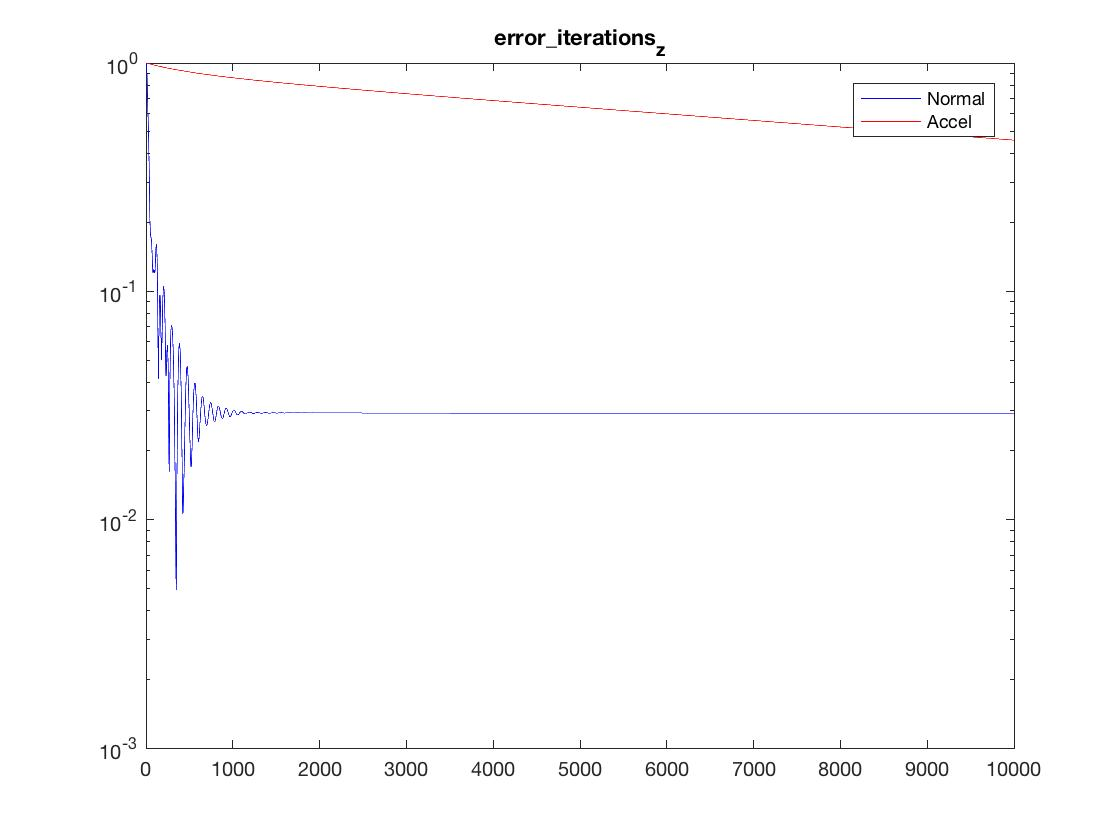
\includegraphics[height = 7.3 cm]{dlm-iterations-log.jpg}
\caption{}
\label{ch5:dlm2}
\end{figure}

\begin{figure}[h]
\centering
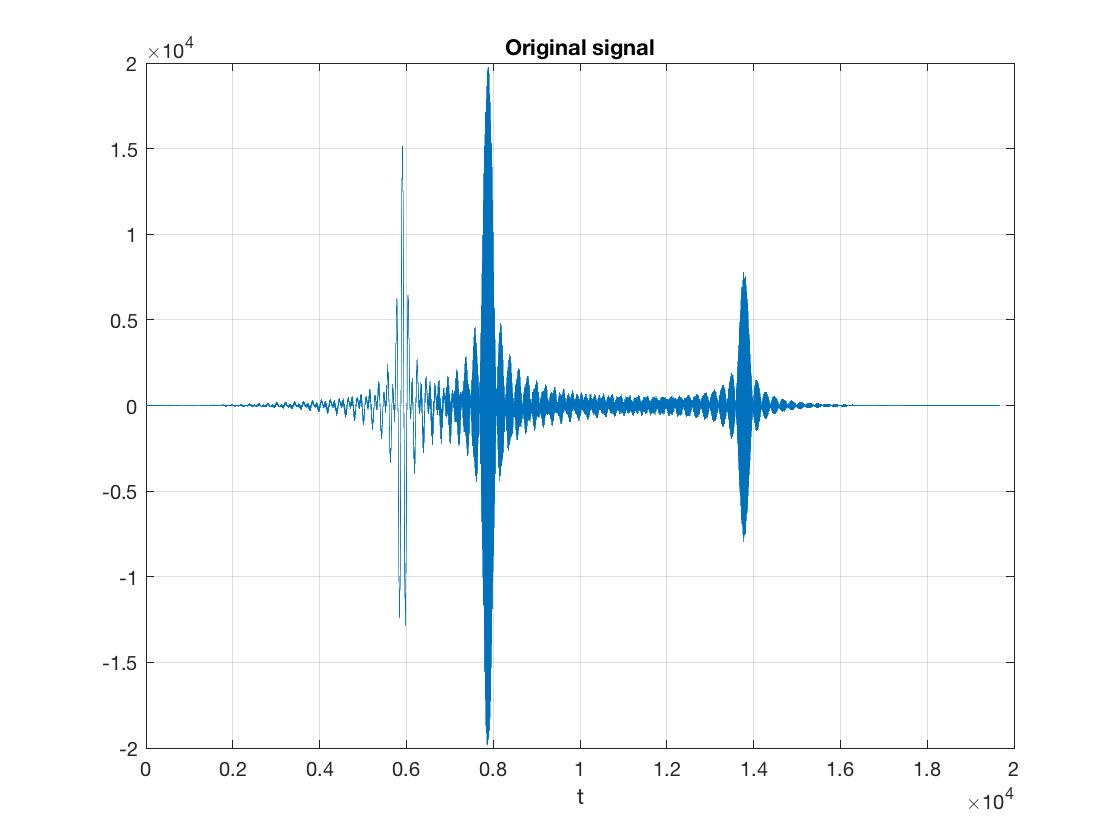
\includegraphics[height = 7.3 cm]{mmv_orig.jpg}
\caption{}
\label{ch5:fig:mmv-orig}
\end{figure}

\begin{figure}[h]
\centering
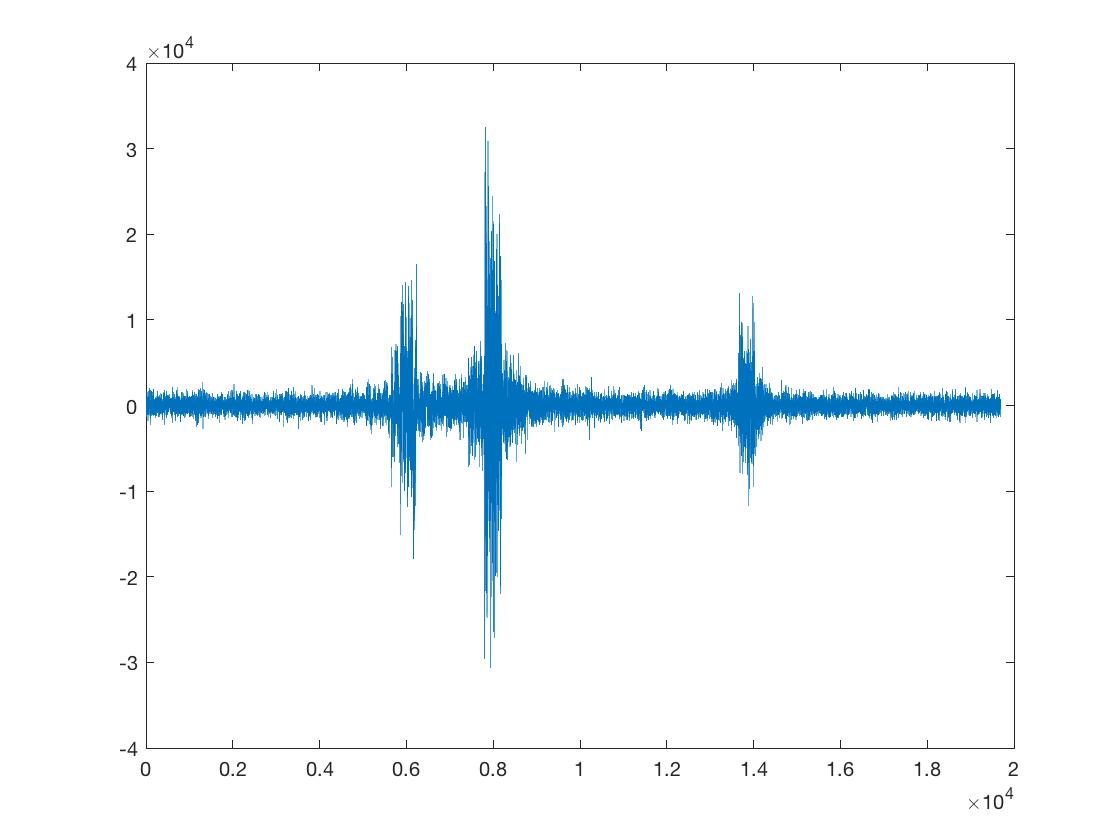
\includegraphics[height = 7.3 cm]{mmv_recon.jpg}
\caption{}
\label{ch5:fig:mmv-recon}
\end{figure}

\begin{figure}[h]
\centering
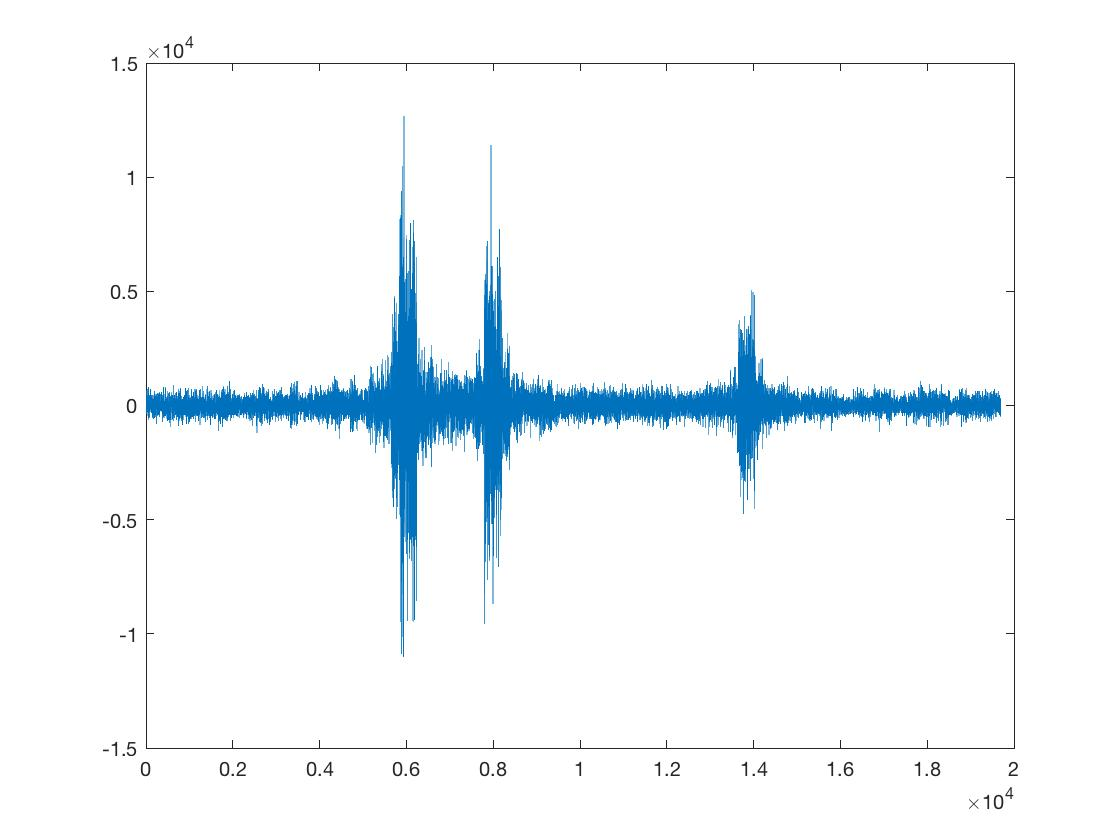
\includegraphics[height = 7.3 cm]{mmv-aty.jpg}
\caption{}
\label{ch5:aty}
\end{figure}

\section{Conclusions}
We have demonstrated an alternating direction algorithm for distributed optimisation with closed forms for the computation at each step, and discussed the statistical properties of the estimation. 

We have simulated the performance of this distributed algorithm for the distributed estimation of frequency spectra, in the presence of additive (white, Gaussian) and multiplicative (frequency flat) noise. We have shown that the algorithm is robust to a variety of SNRs and converges to the same solution as an equivalent centralised algorithm (in relative mean-squared-error).